\documentclass[letterpaper, 10 pt, conference]{ieeeconf}  
\IEEEoverridecommandlockouts                              % This command is only
                                                          % needed if you want to
                                                          % use the \thanks command
\overrideIEEEmargins
% See the \addtolength command later in the file to balance the column lengths
% on the last page of the document

% The following packages can be found on http:\\www.ctan.org
\usepackage{graphics} % for pdf, bitmapped graphics files
\usepackage{epsfig} % for postscript graphics files
\usepackage{amsmath} % assumes amsmath package installed
\usepackage{amssymb}  % assumes amsmath package installed
\usepackage{hyperref} %For hyperlinks
\usepackage{float} % To place graphs
\usepackage{epstopdf}
\usepackage{mathrsfs}


\title{\LARGE \bf
Recommendation Systems for Amazon.com
}
\author{Nikhil Johri, Zahan Malkani, and Ying Wang
}
\begin{document}

\maketitle
\thispagestyle{empty}
\pagestyle{empty}


%%%%%%%%%%%%%%%%%%%%%%%%%%%%%%%%%%%%%%%%%%%%%%%%%%%%%%%%%%%%%%%%%%%%%%%%%%%%%%%%
\begin{abstract}
Modern retailers frequently use recommendation systems to suggest products of 
interest to a collection of consumers. A closely related task is ratings 
prediction, in which the system predicts a numerical rating that a 
user $u$ will assign to a product $p$. In this paper, we build three ratings 
prediction models for a dataset of products and users from Amazon.com. We 
evaluate the strengths and weaknesses of each model, and discuss their 
effectiveness in a recommendation system.

\end{abstract}

%%%%%%%%%%%%%%%%%%%%%%%%%%%%%%%%%%%%%%%%%%%%%%%%%%%%%%%%%%%%%%%%%%%%%%%%%%%%%%%
\section{Introduction}
In this paper, we focus on collaborative filtering methods for recommendations. 
Collaborative filtering is the term applied to techniques that analyze the 
relationships between users and products in a large dataset and make 
recommendations based on existing connections between nodes \cite{bib:recsys}.
One common technique in collaborative filtering is to use existing connections 
to make judgments about similar products and users. Similarity depends only on 
history -- for example, two users may be similar if they have purchased many 
of the same items, so one user's rating can be used to infer a rating for 
another. 

The alternative to collaborative filtering is content filtering, which 
creates features for users and products to assess compatibility. These 
features, which in a book recommendation system might be things like genre or 
subject, will be scored for both users and products \cite{bib:recsys}. This 
makes content filtering highly domain-specific. 
In contrast, collaborative filtering does not need to create such features, 
so it is domain-independent. It is sufficient in collorative filtering to have 
only a matrix of users to products, where each entry in the matrix is some 
scalar indicator of the past relationship between a user and a product.

\subsection{Previous Work}
Collaborative filtering has enjoyed a long popularity in recommendations tasks. 
It was first used commercially in 1992 in a system called Tapestry to 
recommend newsgroup messages to readers \cite{bib:tapestry}. In this system, 
feedback and annotations from existing user-document relationships are used 
to select interesting documents for other users. This system first uses the 
term \emph{collaborative filtering} to indicate that people implicitly 
collaborate by recording their reactions to documents, enabling 
others to make decisions based on those reactions.

Our work is based on two broad categories of collaborative filtering: 
similarity methods and matrix factorization \cite{bib:recsys2}. Similarity 
methods make recommendations by comparing the similarity between users or 
products. In a neighborhood-based similarity model, users are compared to each 
other to determine their nearest neighbors based on their histories. Then, to 
make a prediction for user $u$'s opinion on product $p$, the model looks at the 
opinions of the neighbors of $u$ regarding $p$. Another similarity model is the 
item-based model, which examines item similarity instead of user similarity. 
This approach has been the basis for Amazon's own recommendation engine
 \cite{bib:amazon}. Its advantage is that product similarities can be computed 
offline, and when a user needs a product recommendation, the system performs 
a fast lookup of items similar to ones in the user's history . This speed 
has been beneficial for scalability in Amazon's large purchase network. 

The second type of collaborative filtering is model-based methods, in our case, 
matrix factorization. Matrix factorization does not use history to  model 
similarity like the previously discussed models. Instead, it uses past ratings 
to estimate the parameters of a statistical model for user-product 
relationships \cite{bib:matrixfact}. Users and products are represented as 
vectors in a latent vector space $R^f$. A numerical estimate for the 
opinion of  user $u$ on product $p$ can be obtained by taking the 
cross product of vectors for $u$ and $p$. The values of the latent dimensions 
are learned during a training stage by minimizing the error between known and 
predicted ratings.

Modern recommendation systems are often a combination of 
collaborative filtering, content-based filtering, and matrix factorization. 
One way to create a hybrid model is simply to take the outcomes of several 
approaches and merge them by taking a weighted average. Other 
hybrid techniques incorporate the previously discussed models with other
machine learning methods, such as classification \cite{bib:recsys2}. 
The ways to combine the approaches are numerous, and it is common for 
a recommendation system to incorporate a large number of strategies. 
The top entrants in the Netflix Prize used a hybrid algorithm with over 100 
techniques \cite{bib:bellkor}.

\subsection{Our project}
This project explores some of the most popular ratings prediction methods using 
a dataset from Amazon.com. The dataset, described in Section 
\ref{sec:dataset}, contains product purchase metadata of over 500,000 DVDs, 
music albums, books, and videos. We use both neighborhood-based and 
matrix factorization methods, described in Section \ref{sec:models}, and we 
discuss our findings in in Section \ref{sec:results}. Based on our 
experiments, we hope to shed some light on the nature of the recommendation 
task and the strengths of each of the models.


%%%%%%%%%%%%%%%%%%%%%%%%%%%%%%%%%%%%%%%%%%%%%%%%%%%%%%%%%%%%%%%%%%%%%%%%%%%%%%%
\section{Dataset}
\label{sec:dataset}
We consider two data collections for this project. The first is a set of business
review information from Yelp.com. The second is a collection of Amazon product 
purchase metadata from the Stanford Large Network Dataset Collection.

Yelp.com is a review aggregator site where users review local
businesses. The dataset contains information about several different types of
business venues including restaurants, shops,
nightlife, and beauty spas. A reviewer assigns a 1-5 star rating to a venue and
writes a text review. Other members then have the opportunity to vote on the
usefulness of the review (positive votes only).

Since this dataset is provided by Yelp.com specifically for academic teams to
experiment with algorithms, and not for actual prediction usage, we found the
dataset not large enough to meet our models' training requirements.
Consisting of review information for businesses around 30 universities,
with a total of just 7500 businesses, key characteristics of this set
are in Table~\ref{table:yelpstats}.

As appropriate, we modelled this data using a bipartite graph with users and
businesses as vertices, and the reviews represented as edges.
We built our system to predict the numerical value of the star
rating that a user would bestow upon a business. Unfortunately, we quickly
found that we would not be able to produce robust prediction results from
this dataset as we will discuss in Section~\ref{sec:results}.

\begin{table}[htb]
\centering
\begin{tabular}{|c|c|}
\hline
Users &65,888 \tabularnewline \hline
Reviews &152,327 \tabularnewline \hline
Businesses &9600 \tabularnewline \hline
Reviews per user &Mean = 2.31, Median = 1, STD = 3.83 
\tabularnewline \hline
Reviews per business &Mean = 22.08, Median = 6, STD = 57.4 
\tabularnewline \hline
Average rating given &Mean = 3.64, Median = 4 \tabularnewline
in a review &Mode = 4, STD = 1.21 
\tabularnewline \hline

\end{tabular}
\caption{ Yelp.com Dataset statistics }
\label{table:yelpstats}
\end{table}

The Amazon dataset was considerably larger, with over 
500,000 product entitities, including product title, salesrank, and ratings 
information. For our project, we are concerned with the ratings assigned 
by users to products. We parsed the dataset to a bipartite review 
graph whose nodes are products and users and edges are the ratings given by 
users to products. After extracting only the relevant data, we found many 
duplicate entries where a user $u$ has reviewed a product $p$ several times, 
sometimes assigning different ratings each time. After eliminating the 
duplicates, we reached a dataset with properties shown in 
Table~\ref{table:amazonstats}.

\begin{table}[htb]
\centering
\begin{tabular}{|c|c|}
\hline
Users &1,555,171 \tabularnewline \hline
Reviews &6,285,389 \tabularnewline \hline
Products &548,551 \tabularnewline \hline
Reviews per user &Mean = 4.04, Median = 2, STD = 68
\tabularnewline \hline
Reviews per product &Mean = 11.45, Median = 2, STD = 55.5 
\tabularnewline \hline
Average rating given &Mean = 4.15, Median = 5 \tabularnewline
in a review &STD = 1.2567
\tabularnewline \hline

\end{tabular}
\caption{ Amazon.com Dataset statistics }
\label{table:amazonstats}
\end{table}

The review densities followed a clean power law distribution as can be seen
in Figure~\ref{fig:userhist} for the users and Figure~\ref{fig:producthist}
for the products. As far as the ratings are concerned however, we see in
Figure~\ref{fig:ratings} that they skew towards the high end with a bimodal
general form.

\begin{figure}[h]
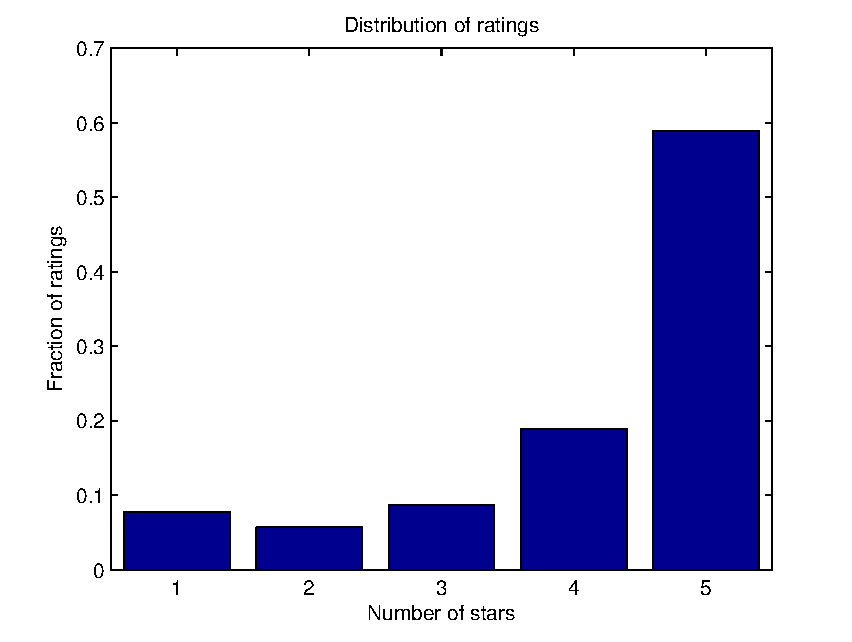
\includegraphics[scale=0.6]{images/ratings.pdf}
\caption{Star rating distribution}
\label{fig:ratings}
\end{figure}

\begin{figure}[h]
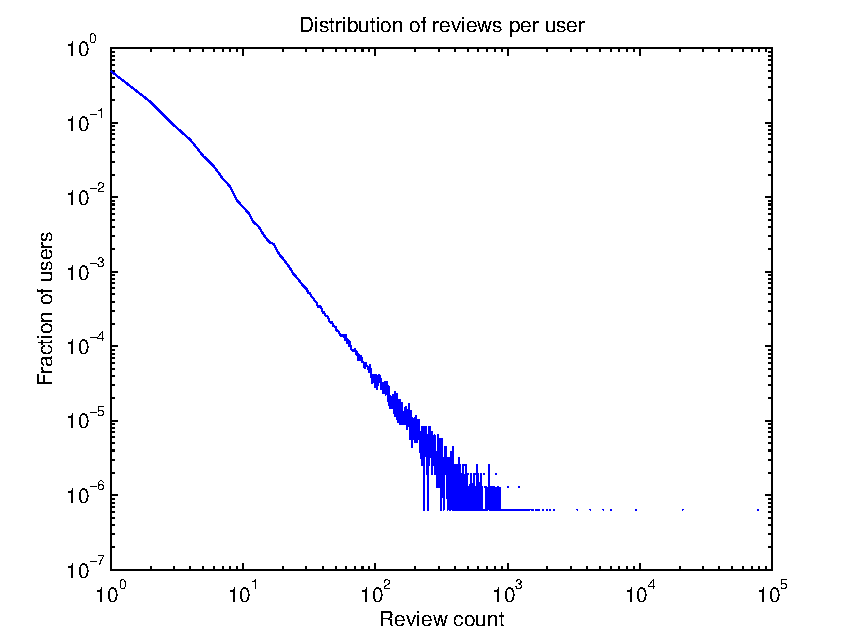
\includegraphics[scale=0.6]{images/user_hist.pdf}
\caption{User review count distribution}
\label{fig:userhist}
\end{figure}

\begin{figure}[h]
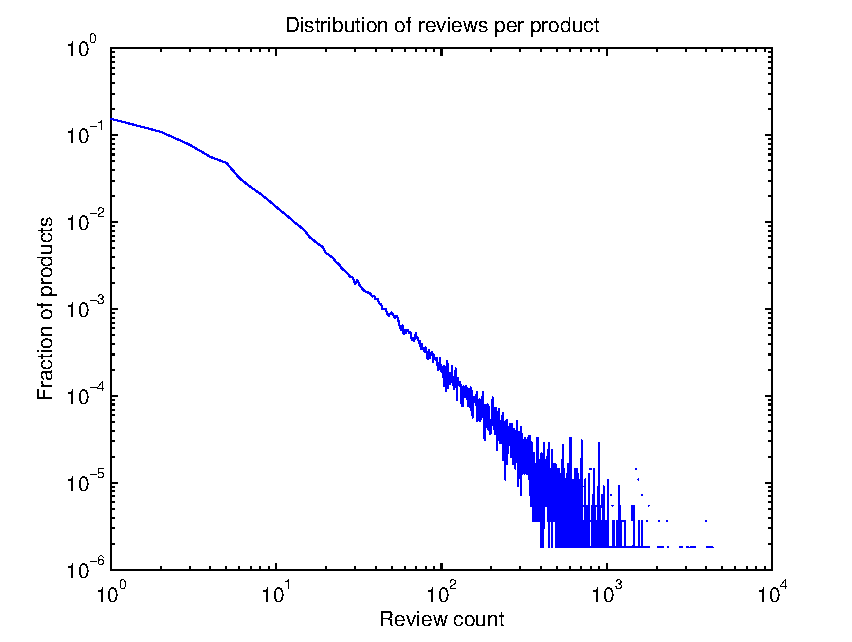
\includegraphics[scale=0.6]{images/product_hist.pdf}
\caption{Product review count distribution}
\label{fig:producthist}
\end{figure}

%%%%%%%%%%%%%%%%%%%%%%%%%%%%%%%%%%%%%%%%%%%%%%%%%%%%%%%%%%%%%%%%%%%%%%%%%%%%%%%
\section{Models}
\label{sec:models}

\subsection{Neighborhood-based model}
\subsection{Modified neighborhood model}
\subsection{Item-based model}
\subsection{Matrix factorization}

%%%%%%%%%%%%%%%%%%%%%%%%%%%%%%%%%%%%%%%%%%%%%%%%%%%%%%%%%%%%%%%%%%%%%%%%%%%%%%%
\section{Results and Discussion}
\label{sec:results}

We report the results of our models on the full Amazon dataset and on our 
high-activity subset. We measure performance over the test sets using 
root-mean-square error. The errors are normalized by dividing by 4, the maximum 
difference between the highest and lowest star ratings possible. However, 
in the interest of preserving granularity for model comparison, predicted
fractional ratings are not rounded to the nearest integer before calculating 
the errors. 

\subsection{Neighborhood-based model}
\subsubsection{Full dataset}
The results of the neighborhood-based model on the full dataset are shown in 
table ?? and Figure ?? below.


\begin{table}[htb]
\centering
\begin{tabular}{|c|c|c|}
\cline{2-3}

\multicolumn{1}{c|}{} & \vbox{\hbox{\strut Neighborhood model}} 
& \vbox{\hbox{\strut Modified }\hbox{\strut neighborhood model}} \tabularnewline \hline
$k$ = 1 & 0.3497 & 0.3870 \tabularnewline
$k$ = 3 &  0.3374 & 0.3544 \tabularnewline
$k$ = 5 & 0.3348 & 0.3448 \tabularnewline
$k$ = 10 & 0.3262 & 0.3397 \tabularnewline
$k$ = 25  & 0.3220 & 0.3346 \tabularnewline
\hline
All other users & \multicolumn{2}{|c|}{?}  \tabularnewline
\hline
Always predict 4 & \multicolumn{2}{|c|}{0.3211}  \tabularnewline
\hline
\end{tabular}
\caption{Neighborhood models, full dataset}
\end{table}

\subsubsection{High-activity dataset}

\begin{table}[htb]
\centering
\begin{tabular}{|c|c|c|}
\cline{2-3}

\multicolumn{1}{c|}{} & \vbox{\hbox{\strut Neighborhood model}} 
& \vbox{\hbox{\strut Modified }\hbox{\strut neighborhood model}} \tabularnewline \hline
$k$ = 1 &  & 0.1397 \tabularnewline
$k$ = 3 &  & 0.1864 \tabularnewline
$k$ = 5 &  & 0.2180 \tabularnewline
$k$ = 10 & & 0.2493 \tabularnewline
$k$ = 25  &  & 0.2645 \tabularnewline
\hline
All other users & \multicolumn{2}{|c|}{}  \tabularnewline
\hline
Always predict 4 & \multicolumn{2}{|c|}{0.3039}  \tabularnewline
\hline
\end{tabular}
\caption{Neighborhood models, full dataset}
\end{table}


\subsection{Item-based model}
\subsection{Matrix factorization}

%%%%%%%%%%%%%%%%%%%%%%%%%%%%%%%%%%%%%%%%%%%%%%%%%%%%%%%%%%%%%%%%%%%%%%%%%%%%%%%
\section{Conclusion}


\begin{thebibliography}{99}

\bibitem{bib:recsys}
Adomavicius, G., Tuzhilin, A. (2005). Toward the next generation of recommender systems: a survey of the state-of-the-art and possible extensions. Knowledge and Data Engineering, IEEE Transactions on , 17(6),  734- 749.

\bibitem{bib:matrixfact}
Bell, R., Koren, Y., Volinsky, C. (2009). Matrix factorization techniques for recommender systems. IEEE Computer 42(8):30-37

\bibitem{bib:bellkor}
Bell, R., Koren, Y., Volinsky, C. (2009). 
The BellKor solution to the Netflix Prize. Technical Report, AT\&T Labs 
Research, 2007b. 
http://www.netflixprize.com/assets/ProgressPrize2007\_KorBell.pdf


\bibitem{bib:tapestry}
Goldberg, D., Nichols, D., Oki, B., Terry, D. (1992). 
Using collaborative filtering to weave an information tapestry. 
Communications of the Association of Computing Machinery, 35(12), 61-70.

\bibitem{bib:amazon}
Linden, G., Smith, B., York, J. (2003). Amazon.com recommendations: Item-to-item collaborative filtering. IEEE Internet
Computing, 7(1), 76-80.

\bibitem{bib:recsys2}
Melville, P., Sindhwani, V. (2010).
Recommender Systems. The Encyclopedia of Machine Learning. 
http://www.prem-melville.com/publications/recommender-systems-eml2010.pdf

\end{thebibliography}

\end{document}
